    % This is samplepaper.tex, a sample chapter demonstrating the
% LLNCS macro package for Springer Computer Science proceedings;
% Version 2.20 of 2017/10/04
%
\documentclass[runningheads]{llncs}
%
\usepackage{graphicx}
\usepackage{hyperref}
% Used for displaying a sample figure. If possible, figure files should
% be included in EPS format.
%
% If you use the hyperref package, please uncomment the following line
% to display URLs in blue roman font according to Springer's eBook style:
% \renewcommand\UrlFont{\color{blue}\rmfamily}

\begin{document}
%
\title{An investigation into the applications of blockchain technology for WoodPlc Ltd}
%
%\titlerunning{Abbreviated paper title}
% If the paper title is too long for the running head, you can set
% an abbreviated paper title here
%
\author{Padraic Wade\inst{1} }
%
\authorrunning{Padraic Wade}
% First names are abbreviated in the running head.
% If there are more than two authors, 'et al.' is used.
%
\institute{
WoodPlc Ltd, Parkmore Galway\\
\email{padraic.wade@woodplc.com}
}
%
\maketitle              % typeset the header of the contribution
%
\begin{abstract}
% The abstract should briefly summarize the contents of the paper in 15--250 words.
In todays world we are hit with an increasing number of technology solutions designed to benifit the end user. One such solution is the use of blockchain technology.
The use of blockchain technology in business to utalise immutable ledgers has become a common talking point in lots of locations with lots of clients coming to us asking what can we do in woodplc to bring some of this technology to prehaps merge into new markets or improve current workflows.
However, this technology as young as it is brings it own sets of challenges to the table. This report summerises the issues and challenges arising from deploying and managing such a network.

\keywords{RDF \and Property Graph \and Graph Database}
\end{abstract}

\section{Introduction}
% Please note that the first paragraph of a section or subsection is not indented. The first paragraph that follows a table, figure, equation etc. does not need an indent, either.

Blockchain technology can be descibed in very simple terms. The concept of an immutable ledger is a simple one but one that has been widely overhyped in all circles. It can be described as a way of processing transactions that can be immutable (as in they cannot be tampered with or edited by an external party) by replicating transactions between machines acting as nodes on a connected network.

We (WoodPlc ltd) has recieved contact from clients who had become interested in blockchain technology and wished to use it in some of the projects we had become involved in. From our intital talks we realsied quickly that our clients had mostly become excited with the prospects of blockchain technology from a PR standpoint rather than what the technology could be used to improve in their current workflows.

We quickly realised that it has become important that we find ways to bring this technology into our workflow but also to find use cases where this technology could be useful in the oil and gas industry which would be our most predomment industry.
Tasks became quickly apparent. We needed to design a solution that would
\begin{itemize}
	\item Be easy for devolpers to interact with.
	\item Hostable on our internal and external cloud systems.
	\item Based off open source technology to reducing licencing costs.
	\item As little self management as possible for end users.
	\item Allow for easy plug and play interaction with our other services.
\end{itemize}

I took the task on to see if I could find a solution that covered the points above and to create a small proof of concept to bring to our business managers to apply for funding for a larger scope project. The scopes of the project were to design and implement the proof of concept that would fit in with the companies internal archtecture guidelines and provide the tools required for devolpers to intergrate into wood web apps and desktop applications.

We will know if we have suceeded in creating a sucessful use case if we have been able to identify a useful aspect of blockchain technology in oil and gas, designed a use case even on a example scale, pushed this to a devolpment enviorment and offered some style of connection for devolpers to take that system and expand it but that work is outside the scope of this project.

After talking to clients both internal and external we realised that none had thought about what exactly they required in the blockchain space. Most wanted something but were unsure about exactly what they required. We quickly relised generic use cases would be the more suitable approach that could be adapted when a suitable project presented itself along with an easy to follow approach for plugging the blockchain application into other projects.


\section{Methodology}

Initally most of the work was done researching different platforms that the blockchain project could be designed on. There were lots of potential canditates such as the dragonchain network ~\cite{DragonChain} which would allow a direct connection into the bitcoin blockchain network, multi concortium ethereum network ~\cite{eth} which would be the industry standard two years ago for designing private networks and NEO ~\cite{neo} a chinese blockchain platform allowing for large scale public deployments. At the time the goal was to find the easiest to deploy on our (at the time totally internal) network. All three code projects were dropped quickly as none offered an easy way to intergrate into our network.

Fast foward to 8 months ago when two major announcements were made from cloud giants aws and azure. Both withen a two month stent launched early wrappers for their semi managed platforms. AWS launched ethereum templates ~\cite{aws} with microsofts azure launching a similar offering months later~\cite{azure} while these were both useful in getting sample projects launched there was still huge barriers getting this code in the hands of our devolpers. The largest being the learning curve.

Most of these new frameworks had some sort of new or modifed programming launguage that run their queries and allow for interaction with their network. Sadly that means it requires a learning curve from the devolpers in order to work with applications and design connections to web apps. Also the most major applications would require extra plugins to make them compatable (for example the web3.js ~\cite{web3} plugin for ethereum contracts) and so adding more complexity to web apps.

Around the same time the first stable offering of the hyperledger foundations fabric ~\cite{hyper} became advailable. Managed by the linux foundation it was setup to create projects to benifit many industries including oil and gas. Fabric was a project origionaly designed by our technical partners IBM and is now managed by the foundation. One of its strongpoints was it was built with business in mind, it is not a public ledger product and contains tools built in in order to allow business to connect quickly and easily. It became the first proper use case for this study.

Azure on the heals of Hyperledger launched a private beta of their workbench program~\cite{bench} this applicaion became the first almost completely azure managed service allowing for a user to launch up a blockchain based off the ethereum framework. This became the second framework to be investigated. 


\section{Technology Review}

As this was an investigation rather than a full blown project we (woodplc) wanted to make sure to push as much of the technology to our providers to allow us to scale and give large SLA's to our clients. Both hyperledger and the azure workbench gave us this option by pushing as much of the management to our providers. 

To give you an idea we run most of our systems on a hybrid cloud so this includes some in azure, aws, ibm cloud and some internal hybrid clouds. 

Hyperledger technology running on ibm's cloud is completly managed (as part of this project most of the work was done there and then transfered back down to files that can be run from a linux machine following the deployment instructions and scripts) for deployment locally in a non production setting. The same applies to the work for the azure blockchain as the deployment scipts included in the source code has work varibles stripped.

The hyperleder fabric application runs on what is known as a consortium. This is where serveral machines contain the same logic in order to process transactions. Whenever a transaction is sent to the network it is first added to a queue. This queue writes it to the ledger of first machine and informs the other machines they need to update their legers with a the same transaction (this causes some awful scaling issues when handling lots of transactions) and then grab the next in the queue. A user can replicate this by having lots of containers on their local enviorment (as detailed in the deployent scripts)


\begin{figure}
\center
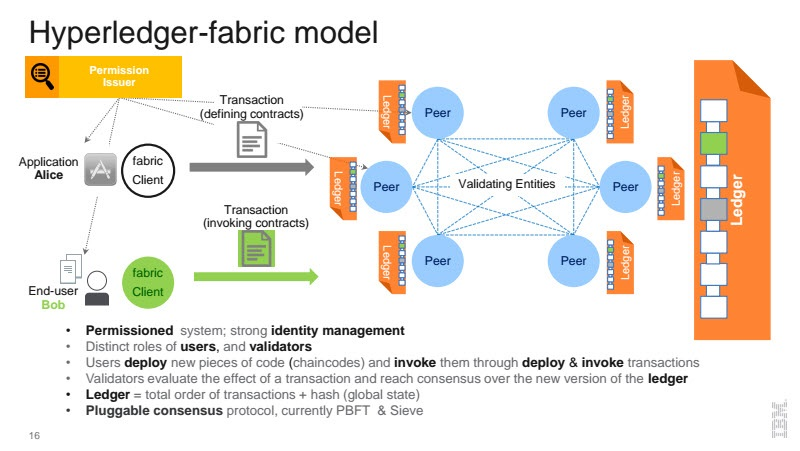
\includegraphics[width=1.0\textwidth]{Hyperledger-Blockchain-model.jpg}
\caption{hyperledger flow}
\label{fig:conversion}
\end{figure}

Azure's blockchain workbench has the same underlying concepts but adds some extra layers to the transactions. The workbench is intergrated with Azure AD, this add some complexity to applications but allows for a greater audit trail on who did what at any time in the project. A user predefined by the workbench owner must sign in and confirm tractions based on the logic presented in the application.
Another unique feature of the workbench is its addition of a SQL db to record transactions. This removes its dependcy of relying on the transaction speed of the consortium. Some may argue this removes the need for the blockchain completly but it helps with handling a lot more concurrent transactions.

\begin{figure}
	\center
	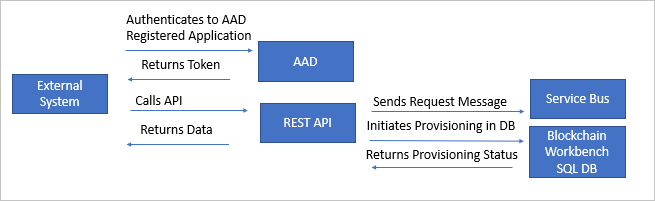
\includegraphics[width=1.0\textwidth]{transactions-ledger.png}
	\caption{azure high level transactions}
	\label{fig:conversion}
\end{figure}

\section{System Design}
These two systems were deployed to three different location for production and two other locations for test. Azure's workbench was both deployed to their fully managed service and an azure edge instance for hybrid work. The hyperledger framework was deployed to both azure, ibm cloud and azure for testing and to docker containers in linux machines for local testing. In these cases most of the work was in an PaaS and in hyperledger IBM it was a completly managed service resulting as a SaaS. 

Azures blockchain workbench contained several conponents that needed to be tailered to work in woodplc network. These included:
\begin{itemize}
	\item an intergration to our work AD to allow for transactions to be signed by a users GUID.
	\item network policies via nsg and vnets to allow us to talk to internal woodplc machines (these machines would be hosted withen azure but wouldnt be publically facing).
	\item intergrations to palo alto firewall and cloudfare routing for traffic management.
\end{itemize}

Hyperledger at a minunium requires several docker containers in order to create its consortium. After that the same conditions apply for outbound traffic such as configuring firewalls and NSG's.

\section{System Evaluation}
Both systems were tested in several ways. Firstly quick tests were taken to see how well transactions could be handled on both networks. Sadly the findings were disappointing as both struggled to process our clients transactions at anything near what a standard database would process. Hyperleder performed worst with it struggling to process more than 2 transactions a second. The use of a database in azure workbench as a buffer helped with inital queries but it soon started to struggle as time went on and its queue got too big to handle. Regardless of whatever amount of data you ingest there would be issues causes by a backlog in the queue of both services. Both services suffered whenever you wanted to return a transaction (ie whenever you wanted to query current status of the blockchain you would be a few minutes behind) and so giving an up to date stats of the current application was difficult.


\section{Conclusion}
In conclusion we found two services we could potentially use but both offer a lot less than what was first expected. They both have shortcommings that would be considered breaking in almost all systems we design in woodplc. The usecases themselves were generic by nature (the use of a supply chain network in both systems) as it was beyond difficult to find a suitable use case that couldnt be done with a database and some logging via azure AD. 
If I was starting this again there would be several things I would do, firstly a huge amount of time was sunk talking to clients about their blockchain needs which wasnt required at all and no suitable usecases could be drawn up. Also looking at a full stack wasnt necessary as most of the work I do is on the archtecture side, creating a more fluid experience for woodplc programmers would have been a more suitable goal.
Overall I wont be recommending we (woodplc) use any blockchain technology for production use until a suitable software stack is designed by the vendors mentioned above or a new party. 


%
% ---- Bibliography ----
%
% BibTeX users should specify bibliography style 'splncs04'.
% References will then be sorted and formatted in the correct style.
%
% \bibliographystyle{splncs04}
% \bibliography{mybibliography}
%
\begin{thebibliography}{8}

\bibitem{DragonChain}
DragonChain network \url{https://dragonchain.com}

\bibitem{eth}
The Ethereum network, \url{https://www.ethereum.org/}.

\bibitem{neo}
Neo blockchain network, \url{https://neo.org/}.

\bibitem{aws}
Amazon web service templates, \url{https://aws.amazon.com/blogs/aws/get-started-with-blockchain-using-the-new-aws-blockchain-templates/}.

\bibitem{azure}
Azure inital proof of stake consortium \url{https://azure.microsoft.com/en-us/blog/ethereum-proof-of-authority-on-azure/}

\bibitem{web3}
Web3.js libary \url{https://github.com/ethereum/web3.js/}

\bibitem{hyper}
HyperLedger Foundation, \url{https://www.hyperledger.org/}


\bibitem{bench}
BlockChain Workbench Azure, \url{https://azure.microsoft.com/en-us/solutions/blockchain/}

\bibitem{source}
Source Code for project, \url{https://azure.microsoft.com/en-us/solutions/blockchain/}
\end{thebibliography}
\end{document}
